\documentclass{article}
\usepackage{tikz}
\usetikzlibrary{shapes,matrix,positioning,arrows.meta,shapes.geometric}
\begin{document}

\begin{figure}
  \centering
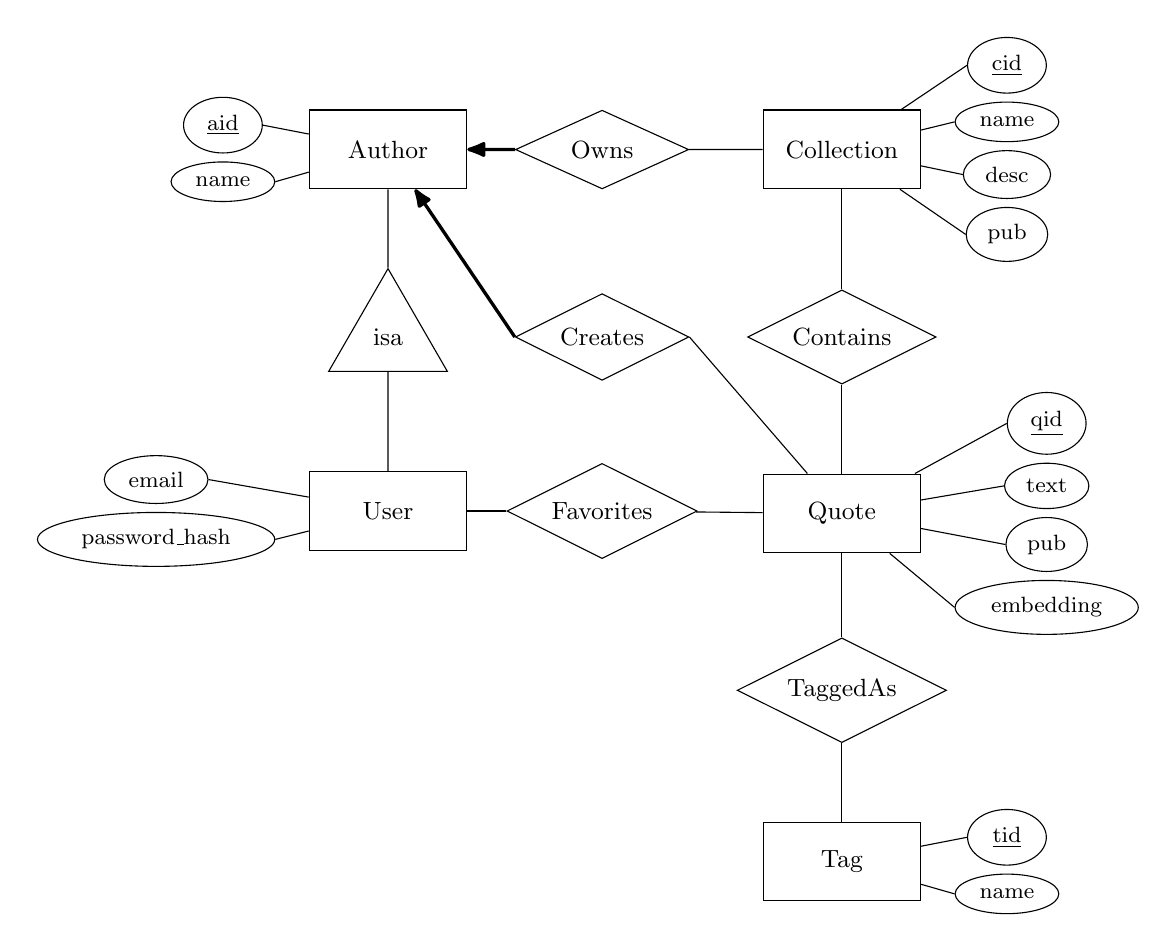
\begin{tikzpicture}
  % Settings
  \tikzset{
    attr/.style={draw, shape=ellipse, minimum width=1cm, minimum height=.5cm, align=center, font=\footnotesize},
    ent/.style={draw, shape=rectangle, minimum width=2cm, minimum height=1cm, align=center, font=\small},
    weak/.style={double,double distance=2pt},
    isa/.style={draw, regular polygon, regular polygon sides=3, minimum width=1cm, minimum height=1cm, align=center, font=\small},
    rel/.style={draw, shape=diamond, aspect=2, minimum width=2.2cm, text centered, align=center, font=\small},
    entrelgrid/.style={matrix of nodes, row sep=1cm, column sep=.5cm, nodes={ent}},
    attrib/.style={matrix of nodes, row sep=.1cm, column sep=.5cm, nodes={attr}},
  }

  \matrix (m) [entrelgrid]{
    \node[name=author] {Author};&\node[rel,name=owns] {Owns};           & \node[name=collection] {Collection};\\
    \node[isa,name=isa] {isa};  &\node[rel,name=creates]{Creates};      & \node[rel,name=contains] {Contains};\\
    \node[name=user] {User};    &\node[rel,name=favorites] {Favorites}; & \node[name=quote] {Quote};          \\
                                &                                       & \node[rel,name=taggedas] {TaggedAs};\\
                                &                                       & \node[name=tag] {Tag};              \\
  };

  % Arrows
  \draw[very thick, -{Latex[round]}] (owns) -- (author);
  \draw[very thick, -{Latex[round]}] (creates.west) -- (author);
  \draw (isa) -- (author);
  \draw (isa) -- (user);

  \draw (owns) -- (collection);
  \draw (contains) -- (collection);

  \draw (contains) -- (quote);
  \draw (creates.east) -- (quote);
  \draw (taggedas) -- (quote);
  \draw (favorites) -- (quote);
  \draw (favorites) -- (user);

  \draw (taggedas) -- (tag);

  % Author attributes
  \matrix (m1) [attrib,left=.3cm of author]{\underline{aid}\\name\\};
  \foreach \i in {1,2} {\draw (m1-\i-1.east) -- (author);}

  % User attributes
  \matrix (m2) [attrib,left=.3cm of user]{email\\password\_hash\\};
  \foreach \i in {1,2} {\draw (m2-\i-1.east) -- (user);}

  % Collection attributes
  \matrix (m3) [attrib,right=.3cm of collection]{\underline{cid}\\name\\desc\\pub\\};
  \foreach \i in {1,2,3,4} {\draw (m3-\i-1.west) -- (collection);}

  % Quote attributes
  \matrix (m4) [attrib,right=.3cm of quote]{\underline{qid}\\text\\pub\\embedding\\};
  \foreach \i in {1,2,3,4} {\draw (m4-\i-1.west) -- (quote);}

  % Tag attributes
  \matrix (m5) [attrib,right=.3cm of tag]{\underline{tid}\\name\\};
  \foreach \i in {1,2} {\draw (m5-\i-1.west) -- (tag);}

\end{tikzpicture}
  \caption{The entity/relationship diagram for QuoteWeave.\label{fig:er}}
\end{figure}

The relations are shown below.

\texttt{Author(aid:int, name:str)}

\texttt{User(aid:int, email:str, password\_hash:str)}

\texttt{Collection(cid:int, aid:int, name:str, desc:str, pub:bool)}

\texttt{Quote(qid:int, aid:int, text:str, pub:bool, embedding:list[float])}

\texttt{TaggedAs(qid:int, tid:int)}

\texttt{Tag(tid:int, name:str)}

\texttt{Favorites(aid:int, qid:int)}

\end{document}
